\subsection{Etapa de Aislación de Señal}

Ahora se debe implementar un circuito auxiliar que provea una aislación galvánica entre los componentes que se sitúan del lado de potencia de la plataforma (como los transistores, diodos, circuito driver, etc.), y los componentes de la parte digital del sistema (como el controlador digital de señales, el circuito de acondicionamiento, etc.).\\

Existen tres partes principales de la plataforma, donde se pasa de la parte digital a la de potencia, donde se requiere algún tipo de aislación:\\

\begin{enumerate}
    \item Entre las salidas PWM del controlador y las entradas de comando de los drivers 2ED21834-S06J de la figura \ref{circuito_driver}.
    \item Para las líneas del bus I\textsuperscript{2}C que comunican al sensor LM5056A de la figura \ref{conexion_LM5056A} (lado de potencia) con el módulo I\textsuperscript{2}C del controlador.
    \item Para la medición de corriente de salida mediante el sensor de efecto Hall TMCS1100A4 de la figura \ref{conexion_TMCS1100}.
    \item Para generar fuentes de alimentación aisladas para los circuitos del lado digital.\\
\end{enumerate}

En este capítulo vamos a tratar las soluciones de aislación para los primeros dos casos. En el tercer caso, el TMCS1100A4, al ser un dispositivo que funciona por medio del efecto Hall, ya tiene aislación incluida en su diseño, por lo que la salida del mismo ya se encuentra aislada del convertidor. Para el cuarto ítem, esto se va a tratar propiamente y en profundidad en la sección de este capítulo dedicada a los circuitos de alimentación de la plataforma.\\

\subsubsection{Tecnologías de Aislación de Señal}

{\Bold\scshape Falta completar esta sección.}\\

\lipsum[1]\\

\subsubsection{Aislación de los Drivers}

Cómo los drivers están conectados directamente a terminales de los transistores de potencia del convertidor, estos se encuentran dentro de la etapa de potencia de la plataforma. Sin embargo, las señales PWM que definen el tiempo y secuencia de conmutación de los transistores provienen del módulo PWM del controlador digital, todo dentro del área digital de la plataforma. Entonces, previo a las entradas de señal de los 2ED21834-S06J se debe interponer algun circuito de aislación de señal, para mantener la separación entre las partes de potencia y digitales.\\

Los requerimientos que la aplicación exige del circuito aislador se presentan en la siguiente lista.\\

\begin{itemize}
    \item Retardo de propagación mucho menor al período $T_s$ de \SI[]{50}[]{\micro\second} de las ondas PWM de excitación.
    \item Tensión pico máxima de aislación superior a los \SI[]{100}[]{\volt}.
    \item Niveles lógicos de salida compatibles con las entradas de los drivers.
    \item Es deseable la utilización de encapsulados pequeños de montaje superficial.\\
\end{itemize}

Para este propósito se eligió utilizar el modelo {\Medium ACPL-P480} de Broadcom, un optoacoplador de un solo canal de alta velocidad, con un \textit{Schmitt trigger} que elimina la necesidad de circuitos externos para acondicionamiento de formas de onda. Algunos de sus parámetros más importantes se muestran en la tabla \ref{tabla:ACPL-P480}.\\

\setlength{\tabcolsep}{8pt}
\renewcommand{\arraystretch}{1.5}
\begin{table}[H]
\begin{center}
    \begin{tabular}{llrrrr}
    {\SemiBold Fabricante} & {\SemiBold Modelo} & $\mathbf{V_{ISO}}$ [\unit{\volt}\textsubscript{RMS}] & $\mathbf{t_{PHL}}$ [\unit{\nano\second}] & $\mathbf{t_{PLH}}$ [\unit{\nano\second}] & $\mathbf{PWD}$ [\unit{\nano\second}]\\
    \hline
    Broadcom & ACPL-P480 & \num{3750} & \num{150} &  \num{110} & \num{250}
    \end{tabular}
    \caption{Especificaciones del optoacoplador modelo ACPL-P480 de Broadcom.\textsuperscript{\cite{ACPL-P480}}}
    \label{tabla:ACPL-P480}
\end{center}
\end{table}

Dónde $V_{ISO}$ es la máxima tensión momentánea soportada entre entrada y salida, $t_{PHL}$ es el retardo de propagación para una transición a nivel lógico bajo, $t_{PLH}$ es el retardo de propagación para una transición a nivel lógico alto, y $PWD$ es la distorsión de ancho de pulso, definida como $|t_{PHL} - t_{PLH}|$.\\

Este dispositivo viene en un empaquetado SMD de seis pines tipo \textit{stretched SO-6} o SO-6 estirado, como el de la figura \ref{encapsulado_opto}. Opera de forma no inversora, es decir que una entrada en alto resulta en una salida en alto, y su etapa de salida está en configuración \textit{totem-pole}, eliminando la necesidad de resistencias de pull-up a la salida. Según el fabricante, la principal aplicación de este modelo es para drivers aislados par gate de MOSFET e IGBT.\\

\begin{figure}[h]
    \centering
    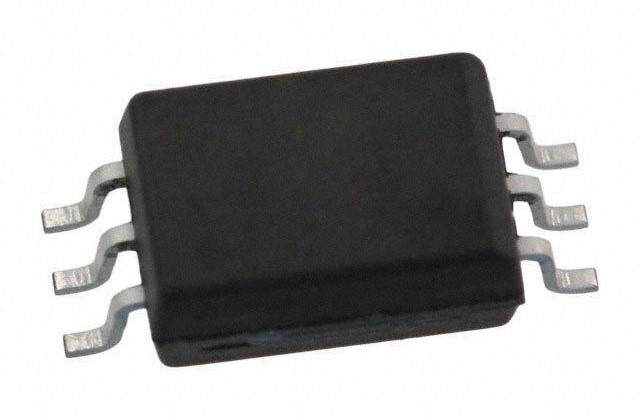
\includegraphics[scale=0.2]{Imagenes/SO6 Stretched.jpeg}
    \caption{Optoacoplador modelo ACPL-P480 de Broadcom, en su encapsulado SMD tipo SO-6 stretched.}
    \label{encapsulado_opto}
\end{figure}

Internamente, el dispositivo consiste de un LED de tipo GaAsP (fosfuro de arseniuro de galio) a la entrada, por el cuál se ingresa la señal. Luego, un detector fotoeléctrico (fotodiodo) junto con un Schmitt trigger (como se mencionó más arriba) capturan la señal luminosa del LED, y la traducen a una señal eléctrica a la salida. Interpuesto entre el LED y el fotodiodo existe un \textit{shield} para reforzar la aislación.\\

\begin{figure}[h]
    \centering
    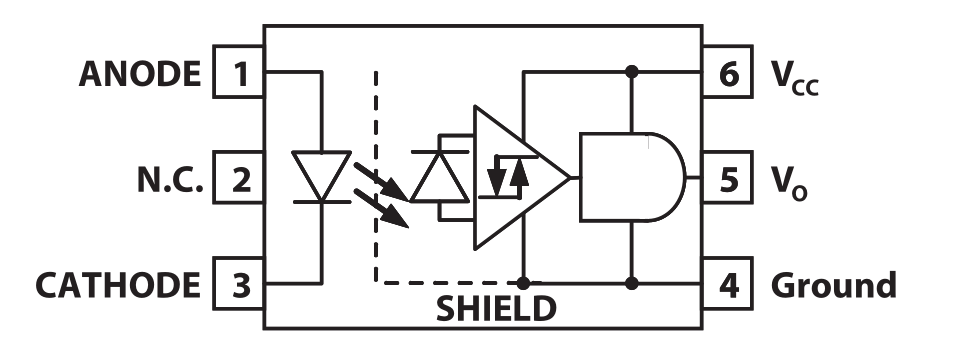
\includegraphics[scale=0.9]{Imagenes/ACPL-P480.png}
    \caption{Circuito interno del optoacoplado ACPL-P480 de Broadcom.}
    \label{circ_interno_opto}
\end{figure}

Entonces, la onda PWM de entrada se conecta al ánodo del LED, con el cátodo conectado a la tierra de señal $GND_D$. La salida del Schmitt trigger en el pin $V_O$ se conecta directamente a la entrada de un dirver, con el pin $Ground$ conectado a la tierra de potencia del primario $GND_1$. El pin de alimentación $V_{cc}$ se conecta a una fuente de \SI[]{5}[]{\volt} como indica la hoja de datos, con un capacitor de bypass entre alimentación y tierra. Cómo cada optoacoplador es de un solo canal, se deben utilizar cuatro ACPL-P480, uno para cada MOSFET del puente, y dos por cada driver.\\

\subsubsection{Aislación I\textsuperscript{2}C}

Como se vió más arriba, el bus I\textsuperscript{2}C es un bus bidireccional de dos cables: uno para la transmisión de datos bidireccional (SDA) y otro que lleva la señal de reloj (SCL), también de manera bidireccional. Sin embargo, los aisladores de señal son dispositivos unidireccionales, por lo que ambas líneas  se debe separar en dos lineas, una para cada dirección.\\

En el caso del LM5056A de la figura \ref{conexion_LM5056A}, la linea de reloj SCL es unidireccional, ya que solo es necesario que el sensor reciba el reloj del controlador; y, para facilitar la aislación, la linea de datos ya se encuentra dividida en dos lineas de entrada y salida (SDAI y SDAO respectivamente). Más adelante, luego del aislador, se debe utilizar algún método para unir las dos líneas de datos en una única linea bidireccional como especifica el protocolo. Con esta información, podemos plantear los requerimientos que debe cumplir el aislador de señal del bus de datos.\\

\begin{itemize}
    \item Debe tener al menos tres canales, con dos en una misma dirección y otro en la dirección opuesta.
    \item Tiempo de propagación mucho menor al período del reloj del bus I\textsuperscript{2}C de \SI[]{100}[]{\kilo\hertz} o \SI[]{10}[]{\micro\second}.
    \item Tensión pico máxima de aislación superior a los \SI[]{100}[]{\volt}.
    \item Niveles lógicos de salida y entrada compatibles con el LM5056A y el controlador.
    \item Es deseable la utilización de encapsulados pequeños de montaje superficial.\\
\end{itemize}

Con estas especificaciones, existen modelos como la serie ISO164x de Texas Instruments, que son aisladores de múltiples canales diseñados específicamente para la aislación de buses I\textsuperscript{2}C: se conecta a sus entradas las lineas bidireccionales y la separación, transmisión a través de la barrera de aislación y unión de las líneas ocurre todo internamente en el circuito integrado. Estos dispositivos ahorrarían la necesidad de implementar un circuito externo para unir las dos lineas de datos del LM5056A, sin embargo, a la hora de adquirir los componentes, y al momento de escribir este informe, se encuentran todos fuera de existencias.\\

Por esta razón, se tuvo que optar por el aislador modelo {\Medium ISO7242C} de Texas Instruments, un aislador de barrera de dióxido de silicio ($SiO_2$) de cuatro canales, con dos canales en cada dirección. Se presenta una tabla con sus principales especificaciones.\\

\setlength{\tabcolsep}{8pt}
\renewcommand{\arraystretch}{1.5}
\begin{table}[H]
\begin{center}
    \begin{tabular}{llrrrr}
    {\SemiBold Fabricante} & {\SemiBold Modelo} & $\mathbf{V_{ISO}}$ [\unit{\volt}\textsubscript{RMS}] & $\mathbf{t_{PHL}/t_{PLH}}$ [\unit{\nano\second}] & $\mathbf{t_{PLH}}$ [\unit{\nano\second}] & {\SemiBold Canales}\\
    \hline
    \makecell[l]{Texas \\ Instruments} & ISO7242C & \num{2500} & \num{42} &  \num{2.5} & \makecell[r]{\num{2} por \\ dirección}
    \end{tabular}
    \caption{Especificaciones del aislador de barrera de $SiO_2$, modelo ISO7242C de Texas Instruments.\textsuperscript{\cite{ISO7242C}}}
    \label{tabla:ISO7242C}
\end{center}
\end{table}

Dónde $V_{ISO}$ es la máxima tensión momentánea soportada entre entrada y salida, $t_{PHL}$ es el retardo de propagación para una transición a nivel lógico bajo, $t_{PLH}$ es el retardo de propagación para una transición a nivel lógico alto, y $PWD$ es la distorsión de ancho de pulso, definida como $|t_{PHL} - t_{PLH}|$.\\

Este dispositivo tiene un encapsulado SMD de dieciséis pines de tipo SOIC-16 como el de la figura \ref{encapsulado_iso}. Tiene la capacidad de ser utilizado con tierras y alimentación aisladas (ya sea de \SI[]{5}[]{\volt} o \SI[]{3.3}[]{\volt}), ya que tiene un pin de tierra y uno de alimentación a cada lado de la barrera de asilación. Además, cuenta con fuciones de habilitación y deshabilitación de canales mediante los pines EN1 y EN2.\\

\begin{figure}[h]
    \centering
    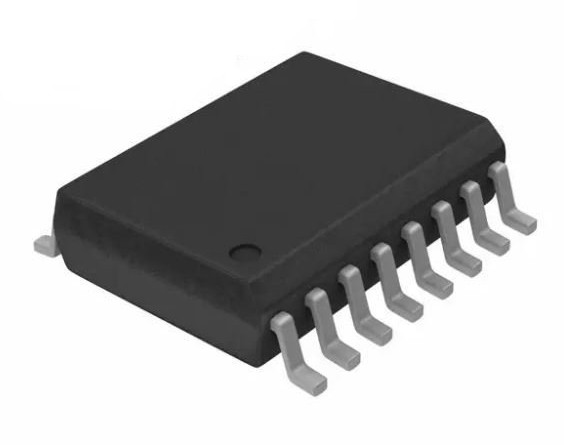
\includegraphics[scale=0.9]{Imagenes/SOIC16.jpg}
    \caption{Aislador de barrera de $SiO_2$ modelo ISO7242C de Texas Instruments, en su encapsulado SMD tipo SOIC-16.}
    \label{encapsulado_iso}
\end{figure}

En nuestro caso, vamos a utilizar tres de los cuatro canales que el dispositivo tiene disponible: un canal en un sentido para SDAO y dos canales en el otro sentido para SDAI y SCL. Para el cuarto canal no utilizado, su entrada se conecta a masa y su salida se deja flotante, como especifica el fabricante. En el lado 1 (lado del LM5056A), se conectan las masas a $GND_1$ al estar del lado de potencia, con la alimentación de \SI[]{5}[]{\volt} conectada al pin VCC1 con su capacitor de bypass en derivación, según especifica el fabricante. Las resistencias de pull-up de \SI[]{4.7}[]{\kilo\ohm} para las líneas de I\textsuperscript{2}C se conectan a la tensión de alimentación de \SI[]{5}[]{\volt}.\\

\begin{figure}[h]
    \centering
    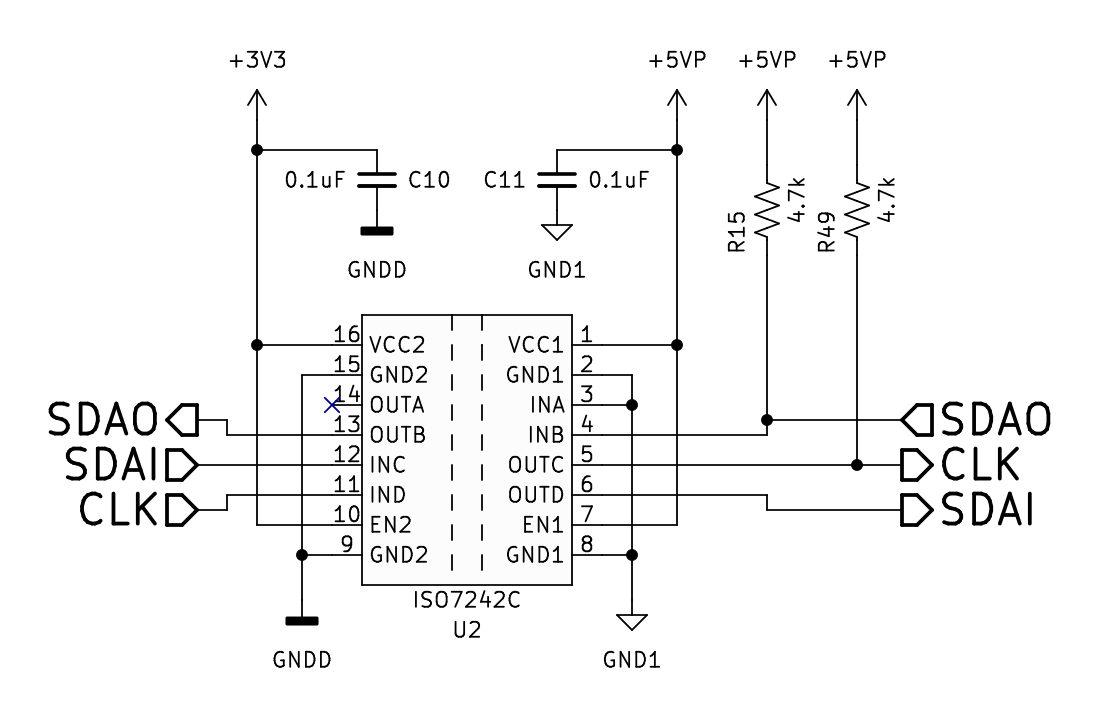
\includegraphics[scale=1.1]{Imagenes/Conexion ISO7242C.png}
    \caption{Conexión del aislador de señal modelo ISO7242C de Texas Intruments para la aislación de un bus I\textsuperscript{2}C.}
    \label{conexion_ISO7242C}
\end{figure}

En el lado 2 (lado del controlador), se conectan las masas a $GND_D$ al estar del lado digital, con la alimentación de \SI[]{3.3}[]{\volt} conectada al pin VCC2, con su capacitor de bypass idéntico al del lado 1. Se eligió alimentar este lado con \SI[]{3.3}[]{\volt} para mantener la compatibilidad con los niveles de tensión de señal del controlador. En ambos lados, los pines de habilitación de canal se conectan a la alimentación, para activar todos los canales (solo se pueden deshabilitar o habilitar todos los canales de una dirección a la vez).\\

\paragraph{Separación de la Línea de Datos}

{\Bold\scshape Falta completar esta sección.}\\

\lipsum[1]\\